\documentclass[a4paper, 10pt]{article}

% Настройки шрифтов
%--------------------------------------
\usepackage[T2A]{fontenc}  % Кодировка шрифтов для русского языка
%--------------------------------------

% Настройки переносов слов
%--------------------------------------
\usepackage{hyphenat}  % Пакет для управления переносами
\hyphenation{ма-те-ма-ти-ка вос-ста-нав-ли-вать}  % Ручные правила переносов
%--------------------------------------

% Настройки языков
%--------------------------------------
\usepackage[english, russian]{babel}  % Поддержка русского и английского языков
%--------------------------------------

% Настройки интерлиньяжа (межстрочного интервала)
%--------------------------------------
\usepackage{setspace}  % Пакет для управления интерлиньяжем
\setstretch{1.3}  % Установка интерлиньяжа в 1.5
%--------------------------------------

% Настройки математики
%--------------------------------------
\usepackage{anyfontsize}  % Пакет для установки произвольного размера шрифта
\usepackage{amsmath, amsfonts, amssymb, amsthm, mathtools}  % Пакеты для математических формул
%--------------------------------------

% Настройки страницы
%--------------------------------------
\usepackage{geometry}  % Пакет для управления геометрией страницы
\geometry{a4paper, portrait, margin=1.5cm, bmargin=1.5cm, tmargin=1.5cm}  % Настройки размеров и полей страницы
%--------------------------------------

% Настройки графики
%--------------------------------------
\usepackage{graphicx}  % Пакет для вставки графики
\usepackage{wrapfig}  % Пакет для обтекания текстом изображений
\usepackage{float}  % Пакет для управления расположением объектов
%--------------------------------------

% Настройки цветов
%--------------------------------------
\usepackage[svgnames]{xcolor}  % Пакет для работы с цветами
\definecolor{codegreen}{rgb}{0,0.6,0}  % Определение цветов для кода
\definecolor{codegray}{rgb}{0.65,0.65,0.65}
\definecolor{codepurple}{rgb}{0.58,0,0.82}
\definecolor{backcolour}{rgb}{0.93, 0.95, 0.96}
\definecolor{keywordcolor}{rgb}{0.23, 0.37, 0.8}
%--------------------------------------

% Настройки для многоколоночного текста
%--------------------------------------
\usepackage{multicol}  % Пакет для создания многоколоночного текста
%--------------------------------------

% Настройки для листинга кода
%--------------------------------------
\usepackage{listings}  % Пакет для вставки и форматирования кода
\lstdefinestyle{mystyle}{  % Определение стиля для листинга кода
    backgroundcolor=\color{backcolour},
    commentstyle=\color{codegreen},
    keywordstyle=\color{keywordcolor}\bf,
    numberstyle=\tiny\color{codegray},
    stringstyle=\color{codepurple},
    basicstyle=\ttfamily\footnotesize,
    breakatwhitespace=false,
    breaklines=true,
    captionpos=b,
    keepspaces=true,
    numbers=left,
    numbersep=5pt,
    showspaces=false,
    showstringspaces=false,
    showtabs=false,
    tabsize=2
}
\lstset{style=mystyle}  % Применение стиля к листингу кода
%--------------------------------------

% Настройки для вставки PDF-файлов
%--------------------------------------
\usepackage{pdfpages}  % Пакет для вставки PDF-файлов
%--------------------------------------

% Настройки для гиперссылок
%--------------------------------------
\usepackage{hyperref}  % Пакет для создания гиперссылок
%--------------------------------------

% Настройки для подчеркивания текста
%--------------------------------------
\usepackage{ulem}  % Пакет для подчеркивания текста
%--------------------------------------

% Настройки для Markdown
%--------------------------------------
\usepackage{markdown}  % Пакет для работы с Markdown
%--------------------------------------

% Настройки для библиографии
%--------------------------------------
\usepackage{biblatex}  % Пакет для работы с библиографией
\addbibresource{literature.bib}  % Указание файла с библиографией
%--------------------------------------

% Настройки для нумерации списков
%--------------------------------------
\renewcommand{\labelenumii}{\arabic{enumi}.\arabic{enumii}}  % Настройка нумерации вложенных списков
\renewcommand{\labelenumiii}{\arabic{enumi}.\arabic{enumii}.\arabic{enumiii}}
\renewcommand{\labelenumiv}{\arabic{enumi}.\arabic{enumii}.\arabic{enumiii}.\arabic{enumiv}}
%--------------------------------------

% Пользовательские команды
%--------------------------------------
\newcommand{\ttgrey}[1]{%  % Команда для выделения текста в серый цвет
  \colorbox{LightGray}{\texttt{#1}}%
}
\newcommand{\bu}[1]{{\color{blue}\uline{#1}}}  % Команда для подчеркивания текста синим цветом
%--------------------------------------

% одинаковые отступы у первого и остальных
\usepackage{indentfirst}
%

% размер формул побольше, все как \[ \]
\everymath{\displaystyle}
%
\begin{document}


\begin{center} % Титульник
    \pagenumbering{gobble}
    \large{Федеральное государственное автономное образовательное учреждение высшего образования}\\
    \Large{Санкт-Петербургский Политехнический Университет Петра Великого}\\
    \Large{Высшая школа прикладной математики и вычислительной физики}\\
    \vspace{6cm}
    \Large{Курсовая работа} \\
    \textbf{\Huge{Построение SV-классификатора (SVM)}}\\

    \vspace{4cm}
    \large

    \centering
    \begin{tabular}{lcl}
        Преподаватель:                       & \hspace{0.6cm} & Павлова Людмила Владимировна \\
        Выполнил студент гр. 5030102/10401:&                &
                                             Прохоров Артём Дмитриевич\\
        Дата:                                &                & \today\\
    \end{tabular}
    
    \vspace{\fill}
    Санкт-Петербург\\
    2025
\end{center}


\large
\clearpage
\pagenumbering{arabic}
\setcounter{page}{2}
\clearpage

\tableofcontents
\clearpage

\section{Постановка задачи}
\textbf{I. SV-подход к решению задачи бинарной классификации:}
\\ Необходимо изложить основные идеи и результаты.
\\(Для \textbf{soft margin SVM} – требуется вывод двойственной задачи $L_D$)
\\


\textbf{II. Практическая часть}
\begin{enumerate}
\item \textbf{Линейно разделимые данные:}
\begin{itemize}
\item Подготовить тренировочную выборку объёмом около 100 объектов,
представляющих точки в двумерном пространстве, которые допускают
линейное разделение.
\item Решить соответствующую задачу квадратичного программирования в
формулировке Вольфа (например, в MATLAB можно использовать функцию
quadprog).
\item Определить опорные векторы (SV) как те, у которых коэффициенты
Лагранжа $a_i \geq tol$, где $ tol = 1e - 3$.
\item Представить:
\begin{itemize}
\item полученные результаты,
\item графическую интерпретацию исходных данных и результатов:
\item разделяющая гиперплоскость и границы,
\item опорные векторы (SV) и пограничные опорные векторы
(BSV), если таковые имеются, и их количество,
\item ширина зазора (margin, M).
\end{itemize}
\end{itemize}
\item \textbf{Нарушенные (зашумленные) линейные данные:}
\begin{itemize}
\item Внести несколько ошибок в обучающую выборку.
\item Построить SV-машину для изменённой (зашумленной) выборки.
\item Исследовать влияние штрафного параметра C на ширину полосы (margin,
M).
\item Вычислить и представить значения M для различных C, например:
C = 0.1, 1, 10, 100, 1000 и т.д.
\item Построить соответствующие графики и визуализации, аналогично п.1.
\end{itemize}
\item \textbf{Нелинейно разделимые данные:}
\begin{itemize}
\item Подготовить выборку объёмом около 100 объектов, которая не допускает
линейного разделения, но разделима нелинейно.
\item Повторить п.1, заменив скалярное произведение на гауссово (радиальное) ядро или другое (см. формулы из лекции).
\item Изучить, как результаты зависят от выбора параметра $\sigma^2$ (или других параметров других ядер).
\end{itemize}
\item \textbf{Нарушенные нелинейные данные:}
\begin{itemize}
\item Внести ошибки в выборку из п.3.
\item Провести аналогичные исследования, как в п.2, для случая нелинейного
разделения:
\item влияние C,
\item ширина зазора M,
\item визуализации.
\end{itemize}
\end{enumerate}


\textbf{III. Работа с реальными данными}
\begin{itemize}
\item Выбрать подходящий по объему датасет из репозитория machine-learning-databases.
\item Выполнить обучение SV-классификатора.
\item Построить визуализацию.
\item Сделать выводы.
\end{itemize}
\section{Алгоритм}

\begin{enumerate}
    \item \textbf{Постановка задачи бинарной классификации}
    \begin{itemize}
        \item \textbf{Данные:} пары $(x_i, y_i)$, где $x_i \in R^n, y_i \in \{ \pm1 \}$
        \item \textbf{Цель:} найти функцию $f(x):R^n\to \{\pm1\}$, минимизирующую эмпирический риск:
        $$R_{emp}[f] = \frac{1}{l}\sum_{i=1}^lL(f(x_i),y_i),$$
        где L — функция потерь (например, $L(f(x),y)=\frac{1}{2}||y-f(x)$).
    \end{itemize}
    \item  \textbf{Линейный SVM для линейно разделимых данных (Hard Margin)}
    \begin{itemize}
        \item \textbf{Гиперплоскость:} $f(x)=(w*x)+b.$
        \item \textbf{Условия:} $$y_i((w*x_i)+b)\geq1, \forall i.$$
        \item \textbf{Оптимизация:} Минимизация $\frac{1}{2}|w|^2$ при заданных ограничениях.
        \item \textbf{Двойственная задача (в формулировке Вульфа):} $$
        \max_{\substack{\alpha}}\sum_{i=1}^l\alpha_i - \frac{1}{2}\sum_{i,j=1}^l\alpha_i\alpha_jy_iy_j(x_i*x_j),$$
        с условиями $\sum_{i=1}^l\alpha_iy_i=0$ и $\alpha_i\geq0.$
    \end{itemize}
    \item  \textbf{Линейный SVM для линейно неразделимых данных (Soft Margin)}
    \begin{itemize}
        \item \textbf{Добавление переменных $\xi_i$} (нарушений границы):$$y_i((w*x_i)b)\geq1-\xi_i, \xi_i \geq 0.$$
        \item \textbf{Оптимизация:} $$\min_{w,b}\frac{1}{2}|w|^2+C\sum_{i=1}^l\xi_i.$$
        \item \textbf{Двойственная задача (Вульфа)} аналогична, но с ограничением $(0 \leq \alpha_i \leq C).$
    \end{itemize}
    \item  \textbf{Нелинейный SVM}
    \begin{itemize}
        \item \textbf{Ядерные функции:} Преобразование $\varphi:X \to H,$ где H - пространство признаков.
        \item \textbf{Примеры ядер:}
        \begin{itemize}
            \item Линейное: $k(x,x')=(x*x')$
            \item Гауссово (RBF): $k(x,x') = e^{-|x-x'|^2/2\sigma^2},$
            \item Полиномиальное: $k(x,x')=(\gamma(x*x')+r)^p.$
        \end{itemize}
        \item \textbf{Решающее правило:} $$f(x)=sgn(\sum_{i=1}^l\alpha_iy_ik(x_i,x)+b).$$
    \end{itemize}
    \item  \textbf{Оценка качества классификации}
    \begin{itemize}
        \item LOO-оценка (Leave-One-Out): $$R_{l00}[f]=\frac{1}{l}\sum_{j=1}^lL(f^j(x_j),y_j),$$
         где $f^j$ обучается на данных без j-го наблюдения.
         \item Кросс-валидация: Разделение данных на k частей и оценка на каждой части.
    \end{itemize}
    \item  \textbf{Преимущества SVM}
    \begin{itemize}
        \item Эффективность в высокоразмерных пространствах.
        \item Использование ядер для нелинейных задач.
        \item Разреженность решения (зависит только от опорных векторов)
    \end{itemize}
    \item  \textbf{Практические шаги}
    \begin{enumerate}
        \item Подготовка данных (масштабирование, обработка выбросов).
        \item Выбор ядерной функции.
        \item Настройка гиперпараметров (например,$C$, $\sigma$).
        \item Обучение и оценка модели.
    \end{enumerate}
\end{enumerate}
\textbf{Вывод двойственной задачи для Soft Margin SVM}
\begin{enumerate}
    \item \textbf{Исходная задача}
    
    Для линейно неразделимых данных вводим переменные ослабления $\xi_i \geq 0:$ $$\min_{w,b,\xi}\frac{1}{2}|w|^2+C\sum_{i=1}^l\xi_i,$$
    с ограничениями: $$y_i((w*x_i)+b)\geq1-\xi_i,\xi_i\geq0, \forall i.$$
    \item \textbf{Функция Лагранжа}

    Добавляем множители Лагранжа:
\begin{itemize}
    \item $\alpha_i \geq 0$ для ограничений $y_i(w*x_i+b)\geq1-\xi_i,$
    \item $\mu_i \geq 0$ для условий $\xi_i \geq 0.$
\end{itemize}

Функция Лагранжа:
$$L(w,b,\xi,\alpha,\mu)=\frac{1}{2}|w|^2+C\sum_{i=1}^l\xi_i-\sum_{i=1}^l\alpha_i[y_i(w*x_i+b)-1+\xi_i]-\sum_{i=1}^l\mu_i\xi_i.$$
\item \textbf{Условия оптимальности (KKT)}

Приравниваем производные к нулю:
\begin{enumerate}
    \item По w:
    
    $\nabla_wL = w-\sum_{i=1}^l\alpha_iy_ix_i=0 \implies w=\sum_{i=1}^l\alpha_iy_ix_i.$
    \item По b:

    $\frac{\partial L}{\partial b}=-\sum_{i=1}^l\alpha_iy_i=0 \implies \sum_{i=1}^l\alpha_iy_i=0.$
    \item По $\xi_i:$

    $\frac{\partial L}{\partial \xi_i}=C-\alpha_i-\mu_i=0 \implies\alpha_i=C-\mu_i.$

    Так как $\mu_i \geq 0,$ то $a_i \leq C.$
\end{enumerate}
\item \textbf{Подстановка в функцию Лагранжа}

Подставляем $w = \sum\alpha_iy_ix_i$ и упрощаем:
$$L=\frac{1}{2}\sum_{i,j=1}^l\alpha_i\alpha_jy_iy_j(x_i*x_j)+C\sum_{i=1}^l\xi_i - \sum_{i,j=1}^l\alpha_i\alpha_jy_iy_j(x_i*x_j)-b\sum_{i=1}^l\alpha_iy_i+\sum_{i=1}^l\alpha_i-\sum_{i=1}^l\alpha_i\xi_i-\sum_{i=1}^l\mu_i\xi_i.$$

Учитывая $\sum\alpha_iy_i=0$ и $\mu_i=C-\alpha_i,$ сокращаем:
$$L_D(\alpha)=\sum_{i=1}^l\alpha_i-\frac{1}{2}\sum_{i,j=1}^l\alpha_i\alpha_jy_iy_j(x_i*x_j).$$
\item \textbf{Двойственная задача}
$$\max_\alpha L_D(\alpha)=\sum_{i=1}^l\alpha_i\frac{1}{2}\sum_{i,j=1}^l\alpha_i\alpha_jy_iy_j(x_i*x_j),$$

с ограничениями:
$$\sum_{i=1}^l\alpha_iy_i=0, 0\leq \alpha_i \leq C, \forall i.$$
\end{enumerate}
\section{Применение алгоритма}

\begin{enumerate}
    \item \textbf{Линейно разделимые данные}

    \begin{enumerate}
        \item Сгенерируем двумерные линейно разделимые данные.
        \item Построим SVM через собственную реализацию:
        \begin{itemize}
            \item вручную сформулируем двойственную задачу в виде задачи квадратичного
программирования (QP);
            \item решим её с помощью cvxopt.
        \end{itemize}
        \item Визуализируем: данные, разделяющую гиперплоскость, margin, опорные векторы.
        
    
\end{enumerate}
    \begin{figure}[H]
        \centering
        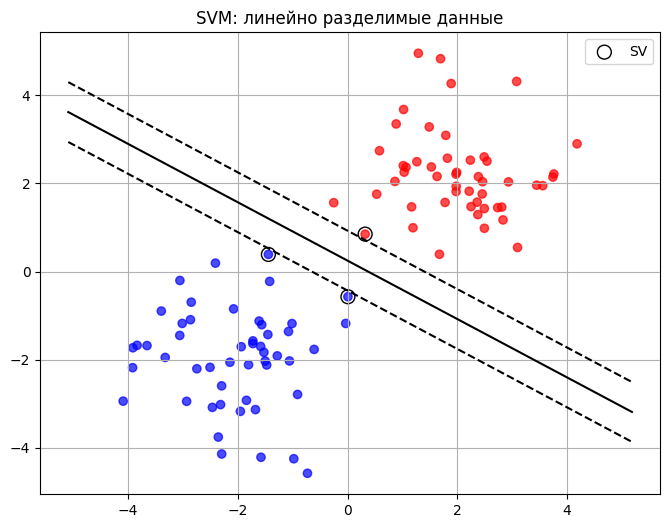
\includegraphics[width=0.75\linewidth]{assets/1.png}
        \caption \centering{Количество опорных векторов: 3
\\ Ширина зазора (margin): 1.3577}
    \end{figure}

\item \textbf{Линейно разделимые данные с шумом}
\begin{enumerate}
    \item Добавить \textbf{шум (ошибки)} в линейно разделимую выборку.
    \item Решим \textbf{soft-margin SVM} с различными значениями C, используя двойственную формулировку.
    \item Визуализируем результаты:
    \begin{itemize}
        \item Разделяющую гиперплоскость,
        \item Опорные и \textbf{пограничные опорные векторы} (BSV),
        \item \textbf{Ширину зазора} для разных C.
    \end{itemize}
\end{enumerate}
    \begin{figure}[H]
        \centering
        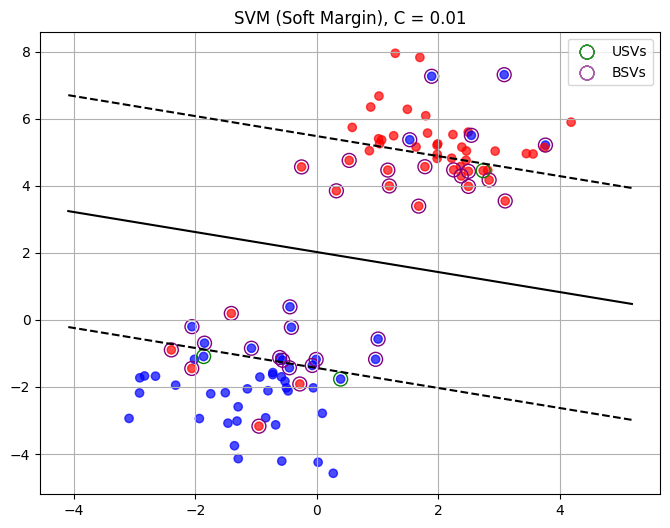
\includegraphics[width=0.75\linewidth]{assets/2.1.png}
        \caption \centering{C = 0.01, Кол-во SV = 38, BSV = 3, Margin = 6.6270}
    \end{figure}
    \begin{figure}[H]
        \centering
        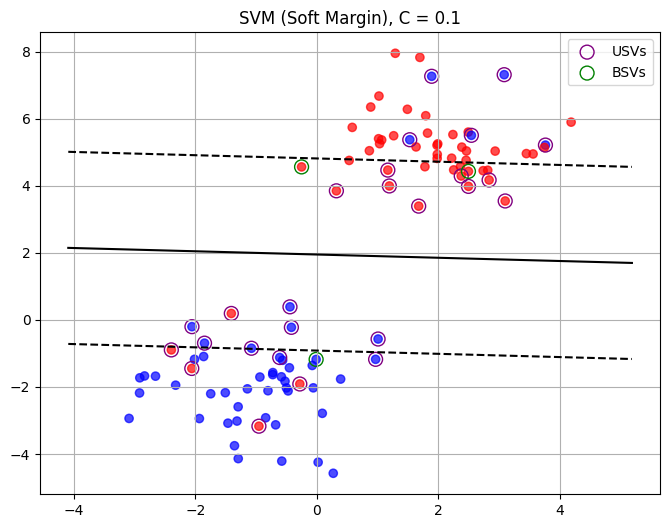
\includegraphics[width=0.75\linewidth]{assets/2.2.png}
        \caption \centering{C = 0.1, Кол-во SV = 29, BSV = 3, Margin = 5.7241}
    \end{figure}
    \begin{figure}[H]
        \centering
        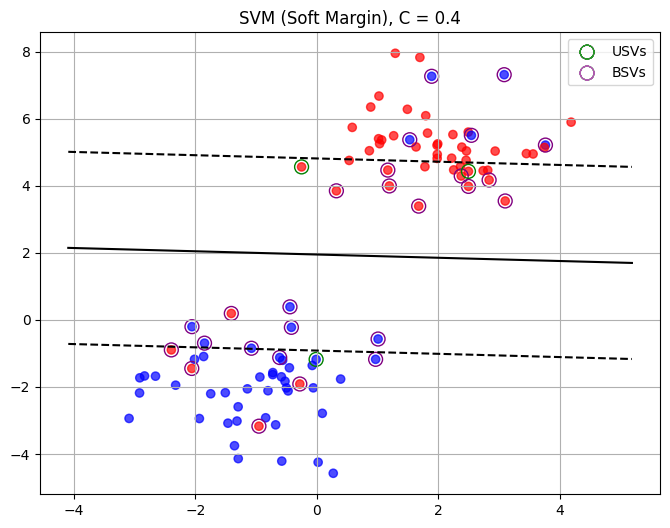
\includegraphics[width=0.75\linewidth]{assets/2.3.png}
        \caption \centering{C = 0.4, Кол-во SV = 29, BSV = 3, Margin = 5.7239}
    \end{figure}
    \begin{figure}[H]
        \centering
        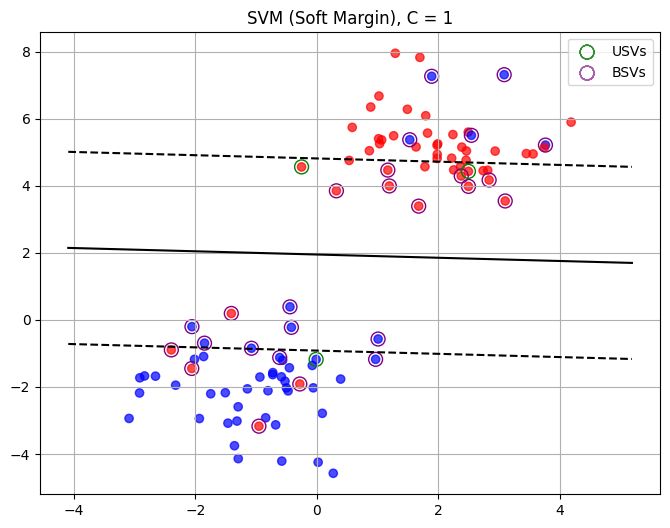
\includegraphics[width=0.75\linewidth]{assets/2.4.png}
        \caption \centering{C = 1, Кол-во SV = 29, BSV = 3, Margin = 5.7248}
    \end{figure}
    \begin{figure}[H]
        \centering
        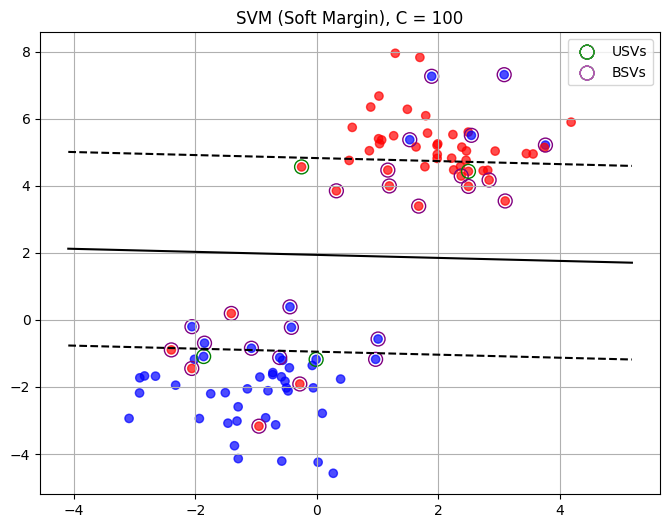
\includegraphics[width=0.75\linewidth]{assets/2.5.png}
        \caption \centering{C = 100, Кол-во SV = 30, BSV = 4, Margin = 5.7688}
    \end{figure}
\item \textbf{Линейно неразделимые данные}
\begin{enumerate}
    \item Сгенерируем \textbf{нелинейно разделимую выборку} (например, кольца).
    \item Решим задачу с помощью \textbf{ядрового SVM}. Используем ядро \textbf{RBF}.
    \item Визуализируем:
    \begin{itemize}
        \item Нелинейную границу,
        \item Опорные векторы,
        \item Эффект параметра ядра ($\gamma$).
    \end{itemize}
\end{enumerate}
    \begin{figure}[H]
        \centering
        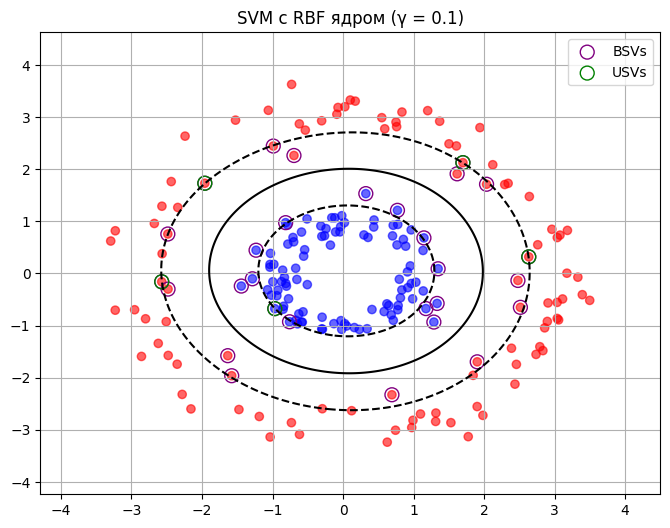
\includegraphics[width=0.75\linewidth]{assets/3.1.png}
        \caption \centering{Gamma = 0.1 Кол-во опорных векторов: 29 Кол-во BSV: 24 Ширина зазора (margin): 0.4286}
    \end{figure}
    \begin{figure}[H]
        \centering
        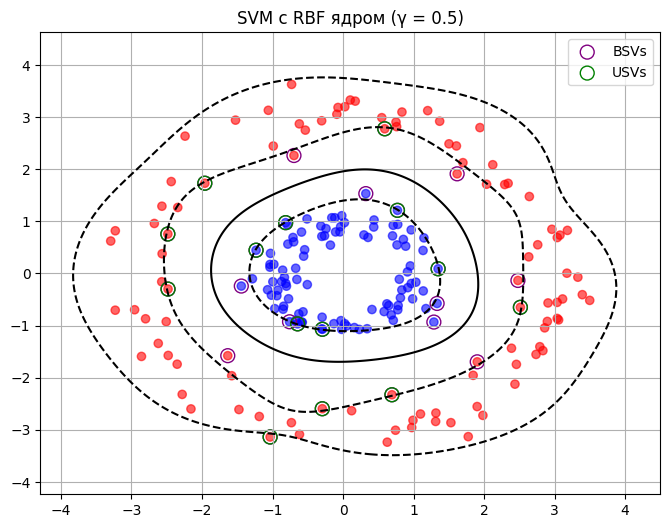
\includegraphics[width=0.75\linewidth]{assets/3.2.png}
        \caption \centering{Gamma = 0.5 Кол-во опорных векторов: 24 Кол-во BSV: 10 Ширина зазора (margin): 0.5331}
    \end{figure}
    \begin{figure}[H]
        \centering
        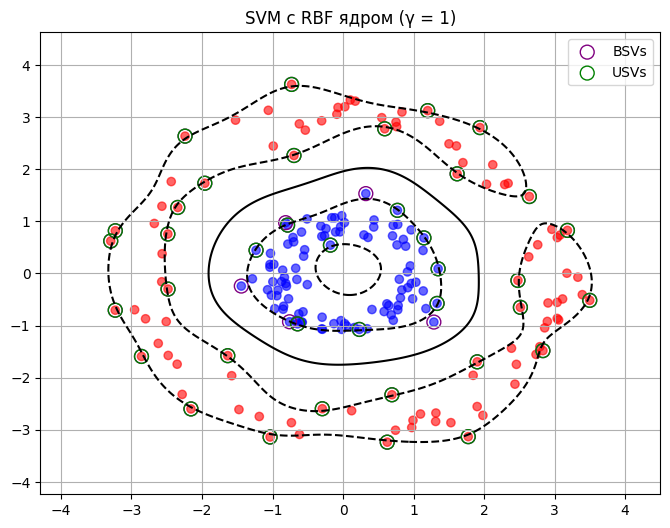
\includegraphics[width=0.75\linewidth]{assets/3.3.png}
        \caption \centering{Gamma = 1 Кол-во опорных векторов: 43 Кол-во BSV: 5 Ширина зазора (margin): 0.5014}
    \end{figure}
    \begin{figure}[H]
        \centering
        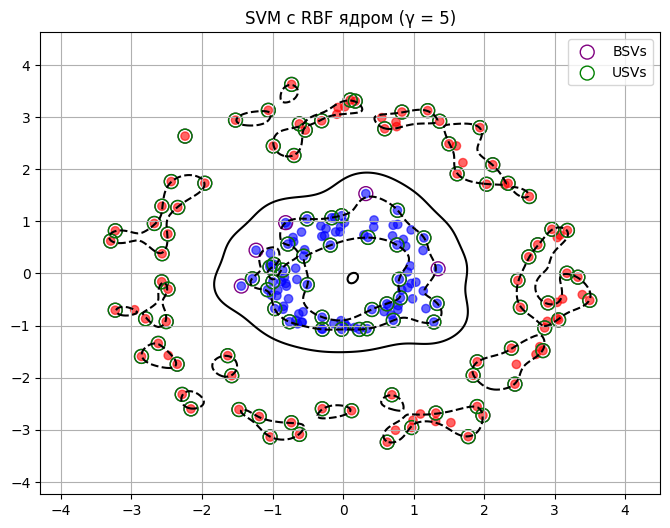
\includegraphics[width=0.75\linewidth]{assets/3.4.png}
        \caption \centering{Gamma = 5 Кол-во опорных векторов: 110 Кол-во BSV: 5 Ширина зазора (margin): 0.3226}
    \end{figure}


\item \textbf{Линейно неразделимые данные с шумом}
\begin{enumerate}
    \item Внесем \textbf{шум (ошибки в метки)} в данные из 3.3 (кольца).
    \item Протестируем \textbf{влияние параметров} на:

    \begin{itemize}
        \item Количество опорных векторов,
        \item Ширину "зазора" M,
        \item Форму границы.
    \end{itemize}
    \item Визуализировать результаты.
\end{enumerate}
    \begin{figure}[H]
        \centering
        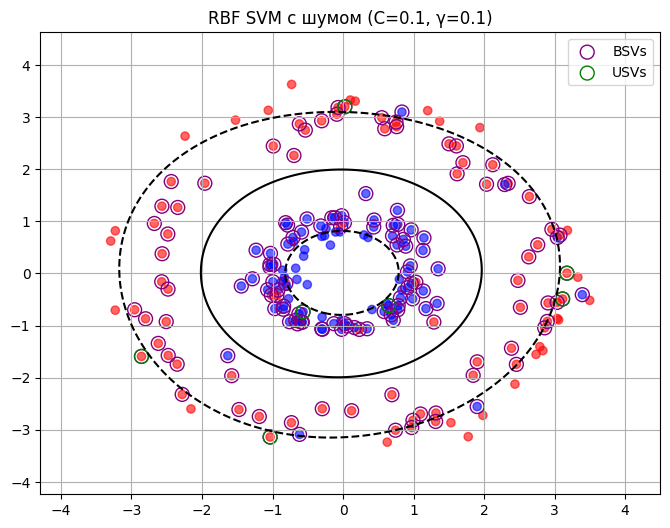
\includegraphics[width=0.75\linewidth]{assets/4.1.png}
        \caption \centering{C = 0.1 | Кол-во опорных векторов: 149 | BSVs: 142 | Оценка зазора (M): 2.484}
    \end{figure}
    \begin{figure}[H]
        \centering
        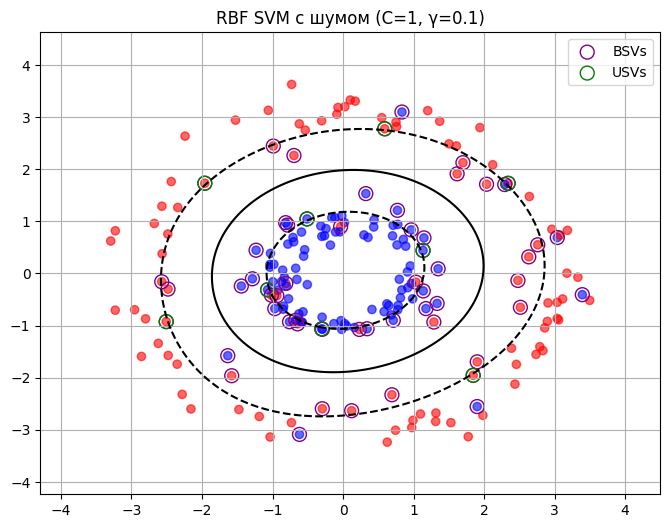
\includegraphics[width=0.75\linewidth]{assets/4.2.png}
        \caption \centering{C = 1 | Кол-во опорных векторов: 59 | BSVs: 50 | Оценка зазора (M): 2.208}
    \end{figure}
    \begin{figure}[H]
        \centering
        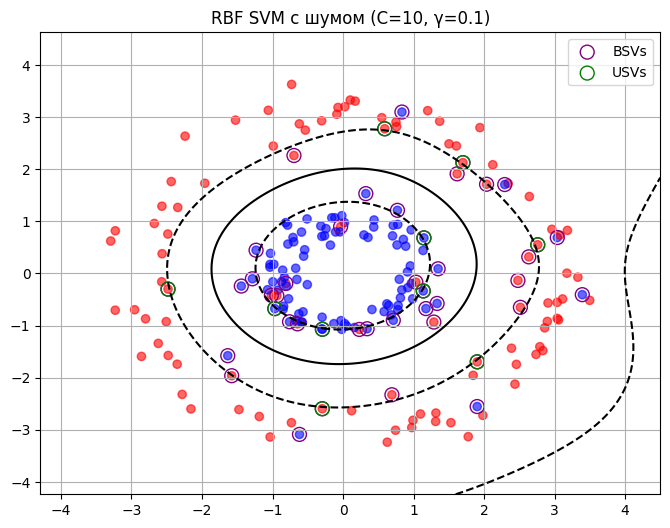
\includegraphics[width=0.75\linewidth]{assets/4.3.png}
        \caption \centering{C = 10 | Кол-во опорных векторов: 44 | BSVs: 34 | Оценка зазора (M): 2.042}
    \end{figure}
    \begin{figure}[H]
        \centering
        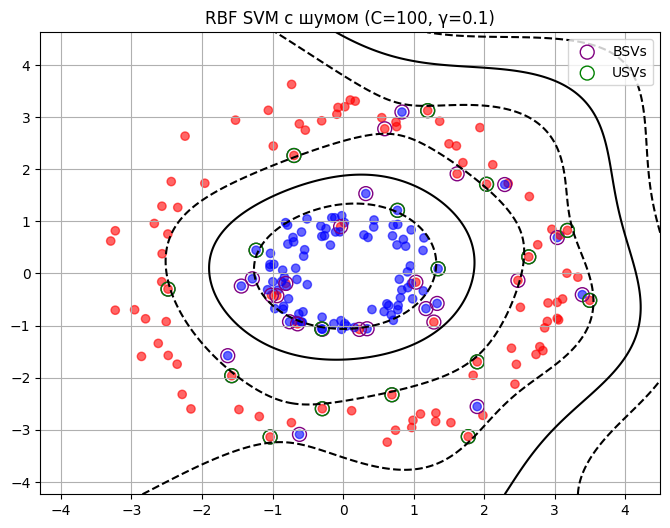
\includegraphics[width=0.75\linewidth]{assets/4.4.png}
        \caption \centering{C = 100 | Кол-во опорных векторов: 43 | BSVs: 26 | Оценка зазора (M): 1.984}
    \end{figure}

Мы можем видеть, что параметры C и $\gamma$ являются параметрами, регулирующими сложность моделей. Чем выше значение С, тем сильнее мы штрафуем модель за ошибки, внутри разделяющей плоскости. То есть, при уменьшении значения параметра C мы сильнее учитываем выбросы при разделении данных на классы. С увеличением же $\gamma$ мы можем строить более сложные разделяющие гиперплоскости, и сильнее подстраиваться под формы расположения данных в пространстве признаков (входных данных).


Наиболее грамотным будет построение модели с помощью жадного или оптимизированного
перебора этих параметров для нахождения оптимальных по итоговому качеству.

\item \textbf{Реальные данные}

Для текущего шага будет использоваться датасет Heart. Он содержит информацию о пациентах, например, их возраст, пол, артериальное давление и уровень сахара в крови. Выход - наличие болезней сердца.



\begin{enumerate}
    \item Загрузим реальные данные heart.
    \item Разделим на тренировочную и валидацонную выборки (80/20).
    \item Стандартизируем их и приведем к виду, удобному для обучения модели.
    \item Решим задачу с помощью ядрового SVM. Используем ядро RBF.
    \item Оптимизируем подбор гиперпараметров через готовую библиотеку optuna, использующую алгоритм байесовской оптимизации.
    \item Измерим качество на валидационной выборке.
\end{enumerate}
Процесс подбора гиперпараметров продемонстрирован ниже:
    \begin{figure}[H]
        \centering
        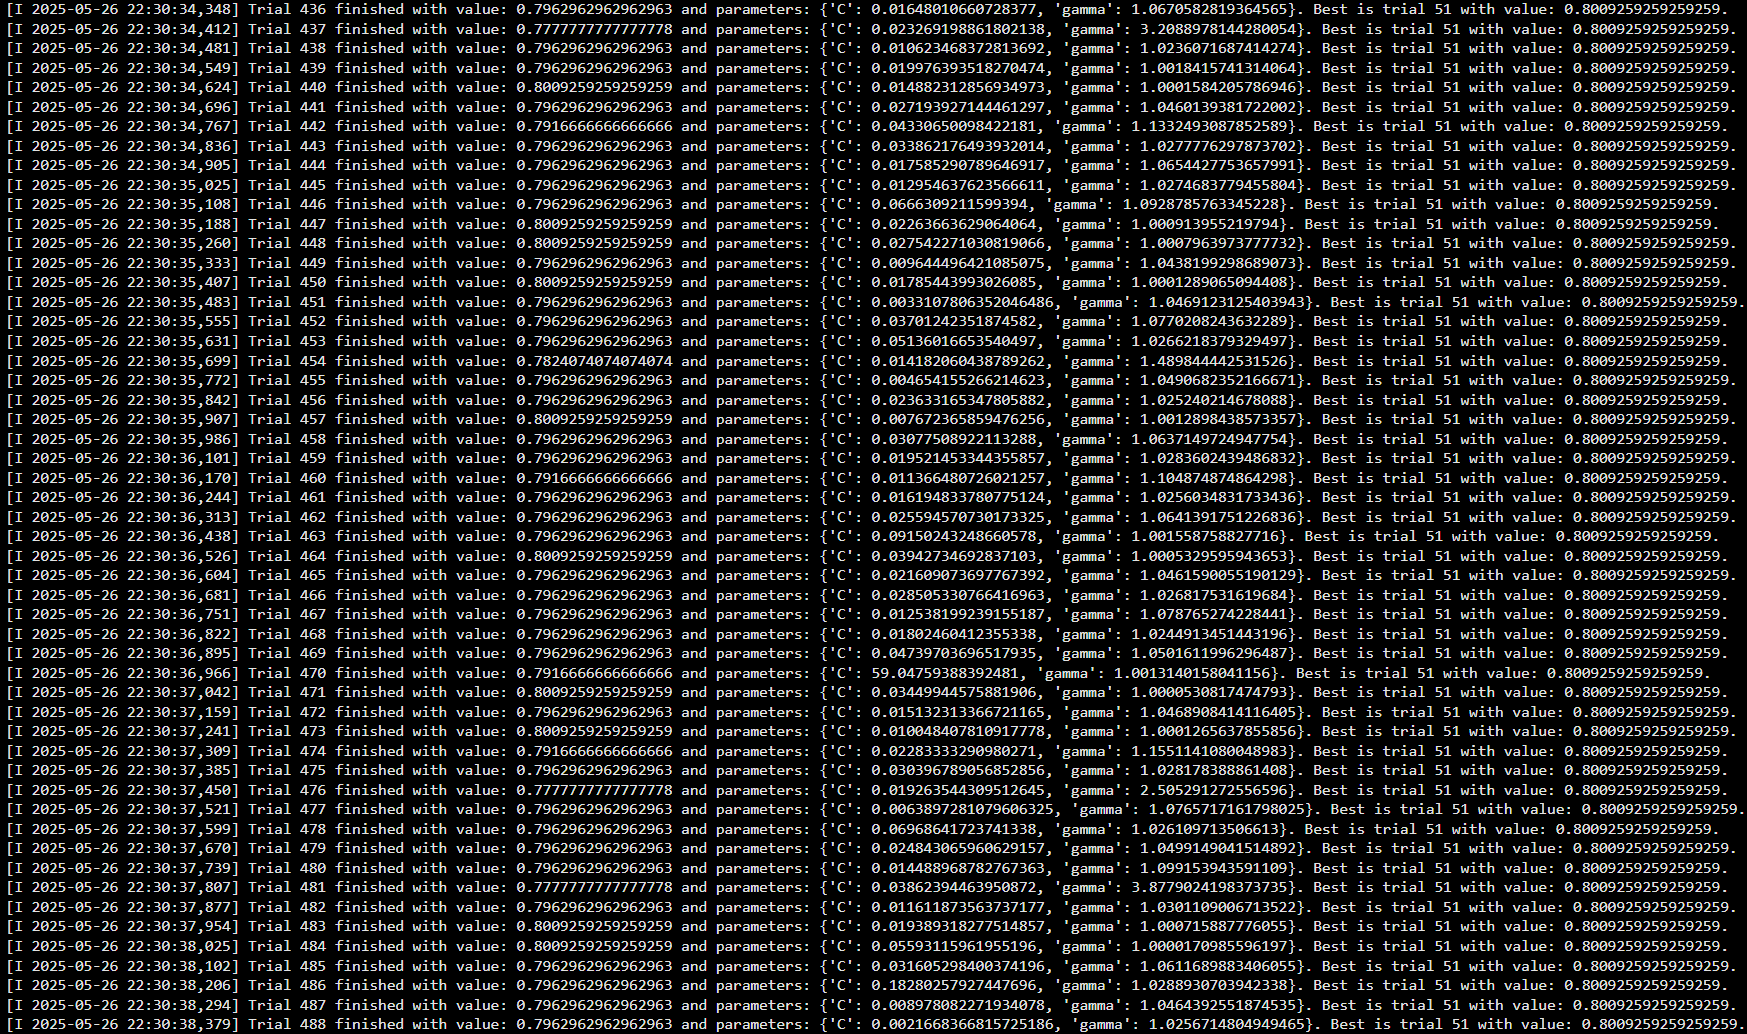
\includegraphics[width=0.75\linewidth]{assets/res1.png}
    \end{figure}
    \begin{figure}[H]
        \centering
        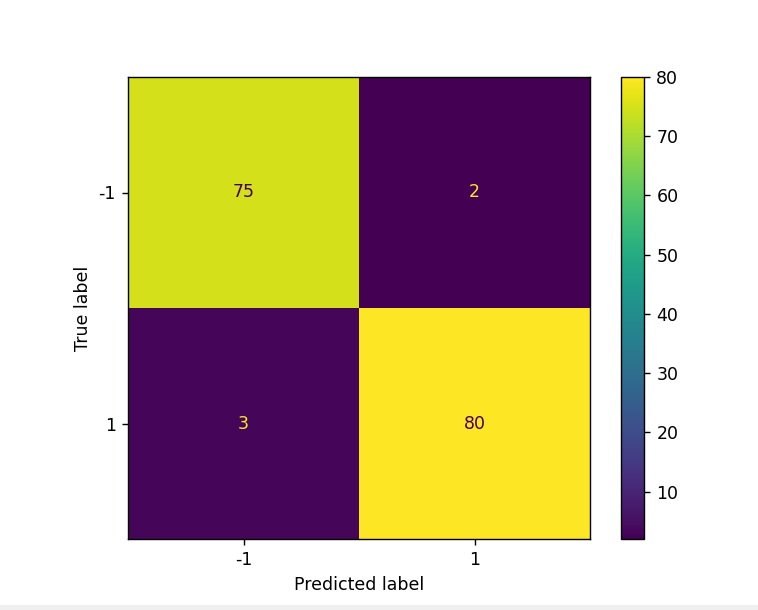
\includegraphics[width=0.75\linewidth]{assets/res2.png}
    \end{figure}
В итоге мы получили модель с точность (accurarcy) равным 0.78 и :
\begin{itemize}
    \item Лучшим С =  0.02910936784038153,
    \item Лучшей гаммой = 1.0006548806873106,
    \item Лучшей точностью = 0.8009259259259259
\end{itemize}

    
Как можно заметить лучшей гаммой было признано значение равное 1. Это указывает на то, что данные хорошо разделены по признакам, но при этом требуется некоторая гибкость при подсчёте. Параметр же регуляризации довольно мал - 0.02, что говорит о том, что данные содержат шум.

\end{enumerate}
\end{document}